\documentclass[twocolumn]{article}
\usepackage[utf8]{inputenc}
\usepackage{blindtext}
\usepackage[paperheight=252mm,paperwidth=174mm,margin=1mm,heightrounded]{geometry}
\usepackage{ulem}
\usepackage{array}
\usepackage{listings}
\usepackage{fvextra}
\usepackage{csquotes}

\usepackage{minted}
%\BeforeBeginEnvironment{minted}{}
%\AfterEndEnvironment{minted}{}

\usepackage{tikz}
\usetikzlibrary{shapes.geometric, arrows}
\usetikzlibrary{positioning}

%% Common TikZ libraries
\usetikzlibrary{calc}

%% Custom TikZ addons
\usetikzlibrary{crypto.symbols}
\tikzset{shadows=no}        % Option: add shadows to XOR, ADD, etc.

\usepackage{color}
\definecolor{light-gray}{rgb}{0.95,0.95,0.95}
\setminted{bgcolor=light-gray}  % this line causes the problem

\setlength{\parindent}{0mm}
\setlength{\parskip}{0mm}

\tikzstyle{string} = [rectangle, rounded corners, inner sep=2mm, text centered, draw=black, fill=red!30]
\tikzstyle{bytes} = [rectangle, rounded corners, inner sep=2mm, text width=, text centered, draw=black, fill=blue!30]
\tikzstyle{int} = [rectangle, rounded corners, inner sep=2mm, text width=,  text centered, draw=black, fill=green!30]
\tikzstyle{arrow} = [thick,->,>=stealth]

\begin{document}

\title{Memory Tracing for Reversing}
\date{}
%\maketitle

\section*{Memory Tracing for Reversing}
\vspace*{-0.5\baselineskip}

When reverse engineering software, we might employ various dynamic analysis techniques throughout the process. These most often focus on what instructions are being executed. For example, we might put breakpoints and observe them being hit, or we might cast a wider net and do a full instruction trace of the program.

Another technique that I have started to appreciate more recently is memory tracing. Here, we focus instead on how the memory is being accessed and what these access patterns can tell us about the software. Broadly speaking, memory tracing answers questions about which memory was accessed, when it was accessed, and what type of operation was performed, i.e. read, write, or execute.

Memory tracing can be done in multiple ways. Hardware breakpoints can be used to watch specific addresses. However, if we want to do a more comprehensive tracing of memory, we typically need some emulation or instrumentation tooling. Popular choices include Intel Pin, DynamoRIO, Frida, and Qiling. In this article, I will go through three examples of when I successfully employed memory tracing.

\vspace*{-0.5\baselineskip}
\subsection*{FlareOn 2018}

\begin{figure}[h]
    \centering
    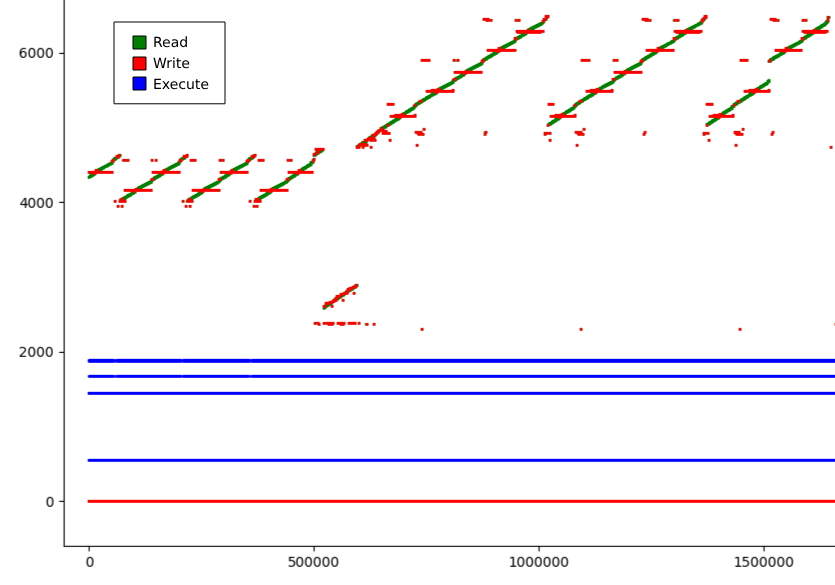
\includegraphics[width=0.9\linewidth]{trace2.png}
    \vspace*{-1\baselineskip}
    \caption{Partial RWX trace of FlareOn 2018/12}
    \label{fig:flareon-trace}
\end{figure}

The final task of the 2018 FlareOn reverse engineering challenge consisted of two nested single-instruction VMs implemented in 16-bit real mode x86. This VM ran a typical crackme where you had to provide the correct input. This code was extremely difficult to grasp, and to process a single byte of the input, about 350 000 x86 instructions were executed. To gain a basic understanding of what was going on, I recorded a trace of the memory accesses using Pin and plotted them\textsuperscript{\ref{fig:flareon-trace}}. Time is on the X-axis, memory space is on the Y-axis, and green, red, and blue represent read, write, and execute, respectively. Since this is a VM, many of the reads actually represent the executed instructions within the VM and thus what we are interested in. From looking at the plot, we can immediately identify loops in the program from the diagonal green lines and even a branch where the green line jumps in the third iteration of the second loop.

\vspace*{-0.5\baselineskip}
\subsection*{VM Deobfuscation}

Last year I was reverse engineering a custom VM. It contained the common construct with a loop that reads the opcode and dispatches the handling to an opcode handler. This is commonly implemented with a loop and a switch-statement or similar but in this case the control flow was heavily obfuscated with opaque predicates and other techniques to make it very difficult to follow. Each handler then read the operands for, and processed, the instruction. To defeat this obfuscation, I emulated the VM with the Qiling framework and traced all memory reads. I had manually identified where the opcode was read at the beginning of the dispatch routine. I recorded any reads at this location, giving me the address of an opcode. I could then trace reads within a small offset of that address and record where they were made from, and their sizes. By repeatedly feeding a crafted memory region with opcodes starting from zero and incrementing them I could extract a full list of opcodes, the number and sizes of their operands, and the location in memory of each opcode handler.

\vspace*{-0.5\baselineskip}
\subsection*{Malware Config Extraction}

A friend reached out and wanted some help with a family of malware. The malware was a botnet agent that reached out to a C2 server to ask for commands. To authenticate the connection, the malware employed a basic challenge-response protocol. The server sends four random bytes, which the malware takes and prepends to a 32-byte key. The SHA2 hash of the resulting 36 bytes is then calculated and sent back to the server. If this key could be automatically extracted it would make it easy for analysts to monitor the botnet's activities. The key was encrypted within the malware binary and decrypted at run-time. Here, I used Qiling again to emulate the malware. I first hooked the connect syscall to make the malware believe it was connected. Then I generated four random bytes and gave them to the malware. By tracing all memory writes, I could then find the address where the random bytes were written, remember it, and record writes adjacent to it. Once all 32 bytes were accounted for, I had the secret key. Compared to static analysis, this technique worked easily across samples on different architectures and various other variations of the malware.

\vspace*{-0.5\baselineskip}
\subsection*{Conclusion}

These are just three examples of how memory tracing can be used in reverse engineering. I encourage you to come up with other applications as well. What I really appreciate about it is that although the same piece of code can look very different when implemented using different languages, on different platforms or with different compilers, a lot of the data access patterns will still be the same. By attacking the data flows instead of the code, many such problems can be bypassed.

%\vfill\null
\end{document}
